%%%%
\chapter{まとめと課題} \label{conclusion}

\section{まとめ}

本研究では、学習者に物理系を定義させるシミュレータである \simname~(\simnamealt) を提案した。
学習者が物理現象を表す方程式を \simname に入力すると、\simname はその方程式に基づく物体の運動を可視化する。学習者は \simname に実装された動作例を参考にすることで、定義した物理系と現実の運動を比較することができたり、次元の異なる物理量の和が存在する不正な方程式を立式すると警告されるなど、正しい物理系を作成するための補助を受ける。
\simname では、物理法則から現象を数式で記述し、シミュレーションに変換するまでの工程も学習者が行うため、従来は授業などで教わる必要があった現実の物理現象と物理法則の間の対応を学習者自らの経験を通して理解することができると考えられる。

\section{今後の課題}

\subsection{評価}

\simname の教育効果を評価する必要がある。高校生を、\simname を用いるグループ・PhET を用いるグループ・座学のグループに分け、pretest と posttest を行う。その結果を Hake~\cite{hake_1998}が導入した Normalized Gain を用いて比較することで、\simname の教育効果を測定できると考える。
% TODO: PhET をどう用いるのか

また、\simname の利点は、現実の運動を確認できるだけでなく、現実の物理現象と物理法則の間の対応を学習者自らの経験を通して理解することができるという点である。そのため、各グループでディスカッションを行い、その内容からどれだけ現実の物理現象を正しく理解できているかを確認することも有効であると考える。

\subsection{方程式計算の支援} \label{6.2.2}

現在、\simname 上に方程式を入力する際、その方程式の導出は学習者が行う必要がある。しかし、移項した際の符号の変え忘れや係数の間違いなど、\simname では検出できないミスが存在する。この作業を以下のような機能を加えてサポートしたい。

\subsubsection{求解の自動化}
$mgh = \dfrac{1}{2}mv_{Ax}^2$ などの入力から自動で $v_{Ax} = \sqrt{2gh}$ と式変形を行うことができれば、計算ミスを防ぐことができる。これは、SymPy の solve 関数などを利用して実装することができる。ただし、自動の式変形では対応できない内容もある。例えば、$mgh = \dfrac{1}{2}mv_{Ax}^2$ を $v_{Ax}$ に関して解いた解は $v_{Ax} = \pm\sqrt{2gh}$ であり、正の場合と負の場合が存在する。このようなときに、学習者に選択させる必要がある。また、式変形を全て自動化してしまうと、学習者自身の式変形に関する能力が成長しない。そのため、自動で求解するかどうかを切り替えられるようにする。

\subsubsection{基本的な公式(運動方程式、力学的エネルギー保存則等)の提供}
基本的な公式を提供し、各値に変数を割り当てるだけ方程式を定義することができるようにする。これにより、学習者の負担を大きく軽減することができる。先述した自動求解を組み合わせることで、適切な公式を選び適切に変数を割り当てるだけで物理系が作成できる。また、公式を解説付きで一覧にしたり、公式の検索機能をつけることで、公式を覚えきれてない初学者に対してもサポートができる。


\subsection{場への対応} \label{6.2.3}
重力場・電場・磁場などのベクトル場や、ポテンシャルなどのスカラー場の可視化に対応することを考えている。場を可視化することができれば、万有引力の法則やクーロンの法則などに従う物体の運動をよりよく表現することができる。図~\ref{field_example} は、matplotlib を用いてベクトル場を可視化する例である。学習者にベクトル場を表す関数を定義させることも可能だが、学習者が生成した物体から学習者が指定した場を自動的に生成し描画することで、より手軽に利用することができる。

\begin{figure}[htb]
  \centering
  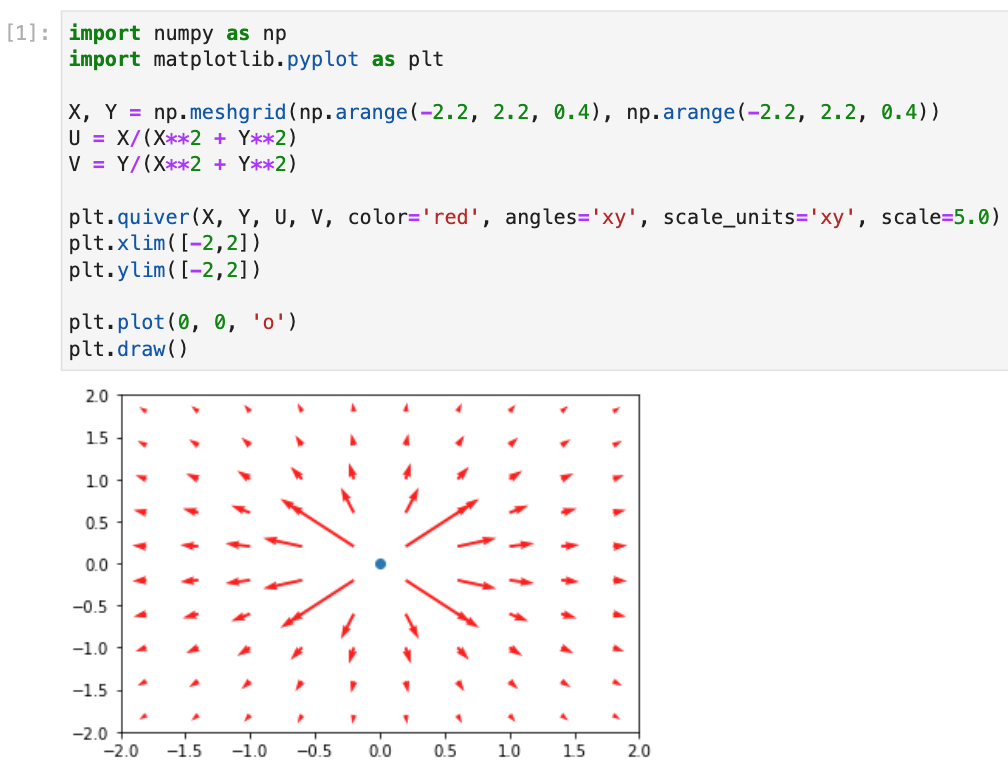
\includegraphics[width=0.9\linewidth]{work/field_example.png}
  \caption{ベクトル場の可視化例} \label{field_example}
\end{figure}


% 現在の \simname の構成は、力学に特化した設計を行なっている。例えば、物体を追加した際の次元付き変数の生成や観測ペインでの位置や速度の可視化である。一方、高等学校で扱う物理には、音や光などの波動分野、回路や電場・磁場などの電磁気分野なども存在する。そのため、これらの分野にも対応できるようにしたい。
%TODO: 具体的な課題・アイデア

% 現在の \simname の構成は、物体を追加した際の次元付き変数の生成や観測ペインでの可視化において単純な力学を重視した設計を行なっている。より多くの現象に対応するため、以下の要素などを加えたい。

% \subsubsection{相対速度への対応}
% 流れのある川の上をボートが渡る際など、

% \subsubsection{場への対応}
% 重力場を可視化することができれば、万有引力の法則などを表現することが可能である。また、電場・磁場を加える事で、電磁気的な力を受ける物体の運動も表現できる。


\subsection{三次元空間への対応}
現在は二次元のグラフで描画を行なっているが、電磁気的な力を受ける場合などは三次元的な運動をする事が多いため、三次元空間を扱う必要がある。方程式の定義や数値計算は単純に拡張すれば良いが、現在の matplotlib を用いた可視化では三次元空間に対応することは容易ではないため、可視化手法を検討する。


